
\section{Evaluation}

\subsection{Data-Driven Performance Engineering}
\subsubsection{Sparse-Sparse Matrix Multiply (SpGEMM)}
\changwan{
Explain what is SpGEMM. why SpGEMM hard? (not sure)
three approaches. Asym time complexity?
}




\help{The main points of this section are:}

\help{1. summarize the difference between inner, gustavson, and outer, cite gamma but this also needs to stand on it's own}


\help{2. Explain why bytemap temporary makes sense for gustavson, but not for outer or inner}

\help{3. Point out that TACO does not even support outer product because it does not support scatter into 2D workspace}

\help{4. Take a look at the figure and point out that Finch is competitive with TACO on inner and gustavson, and that for outer product we see what we would expect from TACO: i.e. Finch Outer with dense performs similarly to TACO with dense, and Finch Outer with sparse performs much better as the matrix size increases.}

\help{5. point out that for the large matrices finch is competitive with TACO for gustavson}.

\help{6. explain the features of "datastructure-driven programming" that are used here in this problem. i.e. explicit temporary, bytemap format, transpositions}.
\begin{figure}
	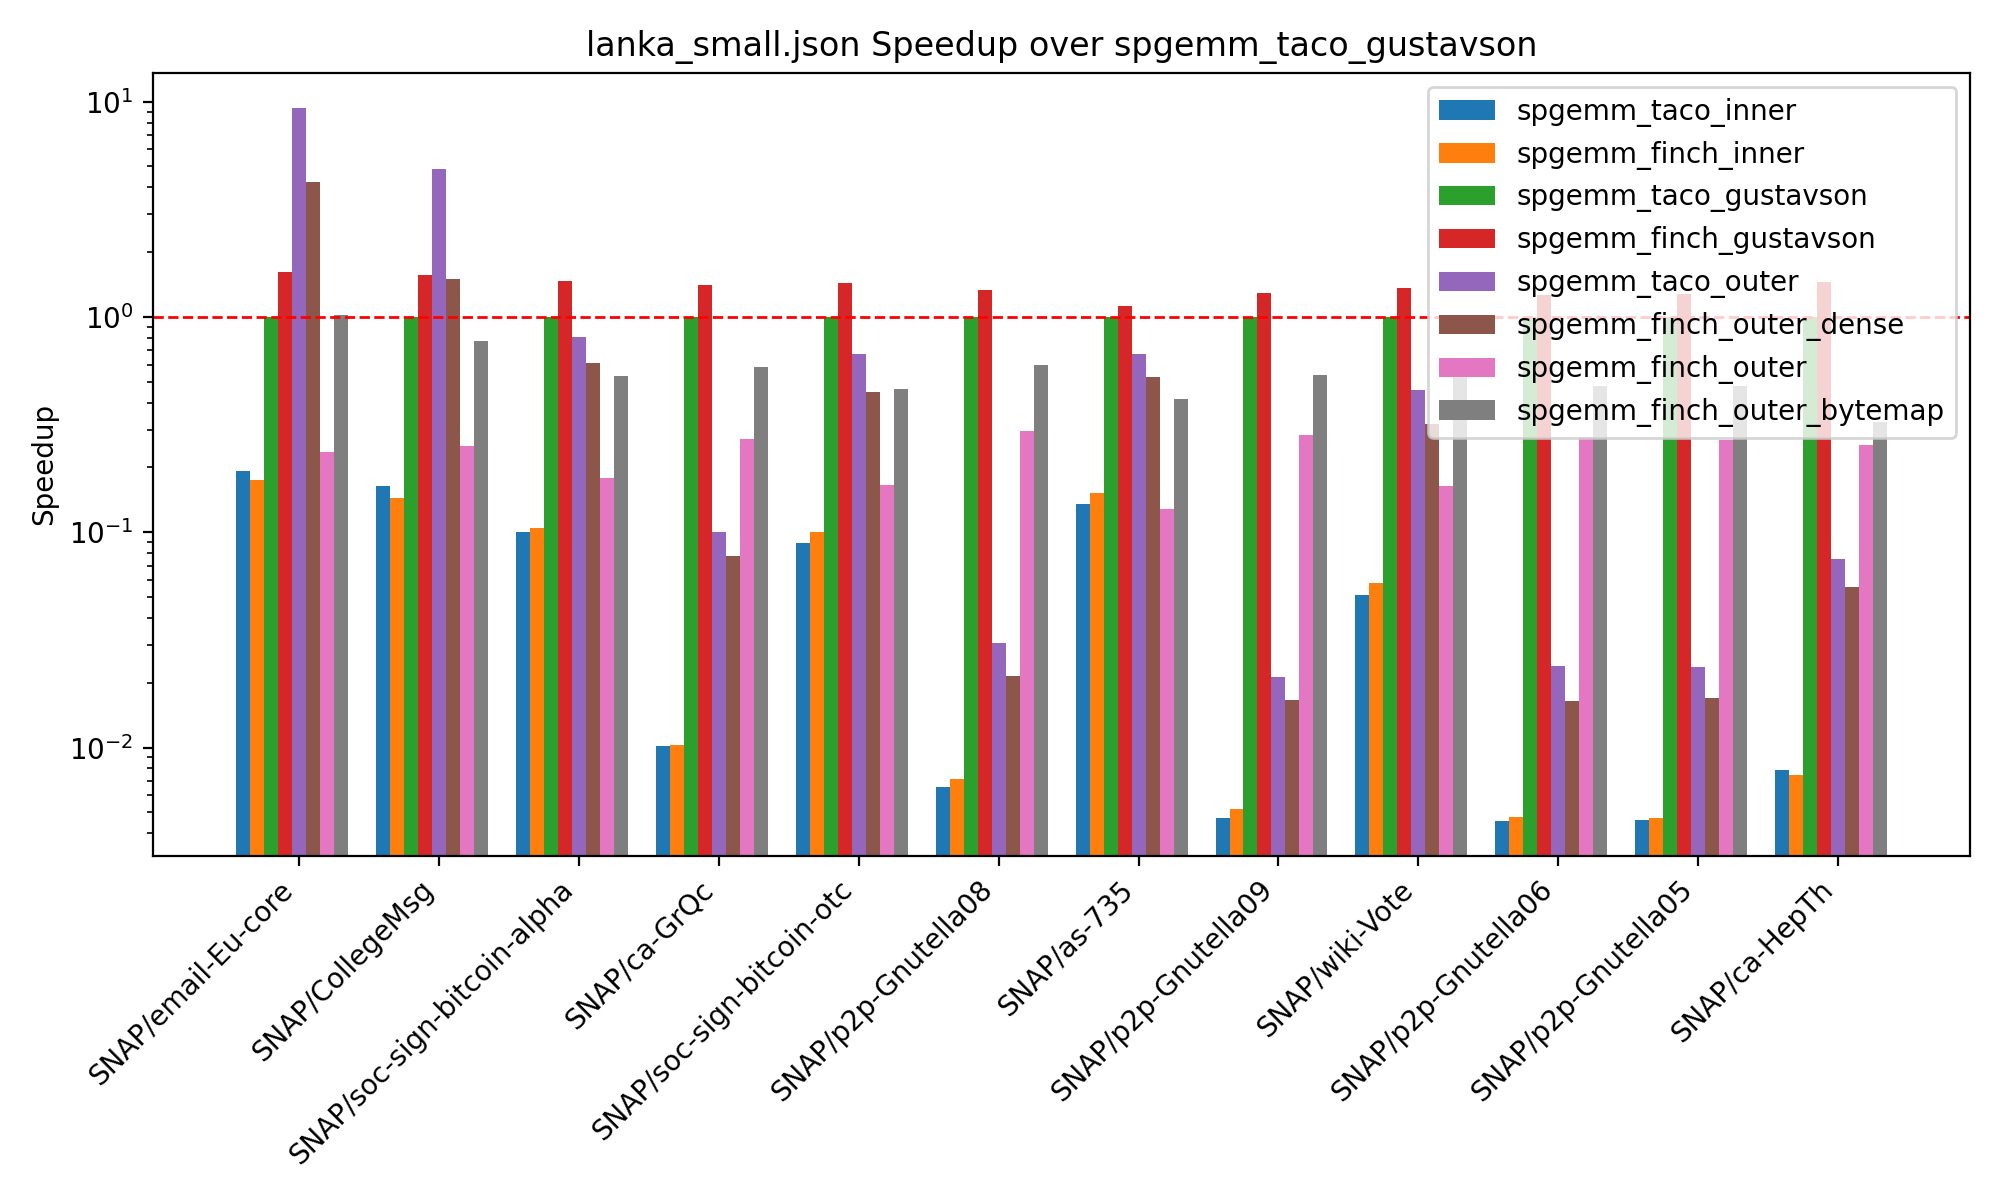
\includegraphics[width=\linewidth]{spgemm_small_speedup_log_scale.png}
    \caption{A comparison of several matrix multiplication algorithms between Finch and Taco smaller matrices, ordered from small to big dimension. Note that inner products necessarily requires $O(n^2)$ work and taco's outer products format is dense. Finch can use a sparse outer products format and thus has an asymptotic advantage that becomes evident as the output dimensions grow.}
\end{figure}

\begin{figure}
	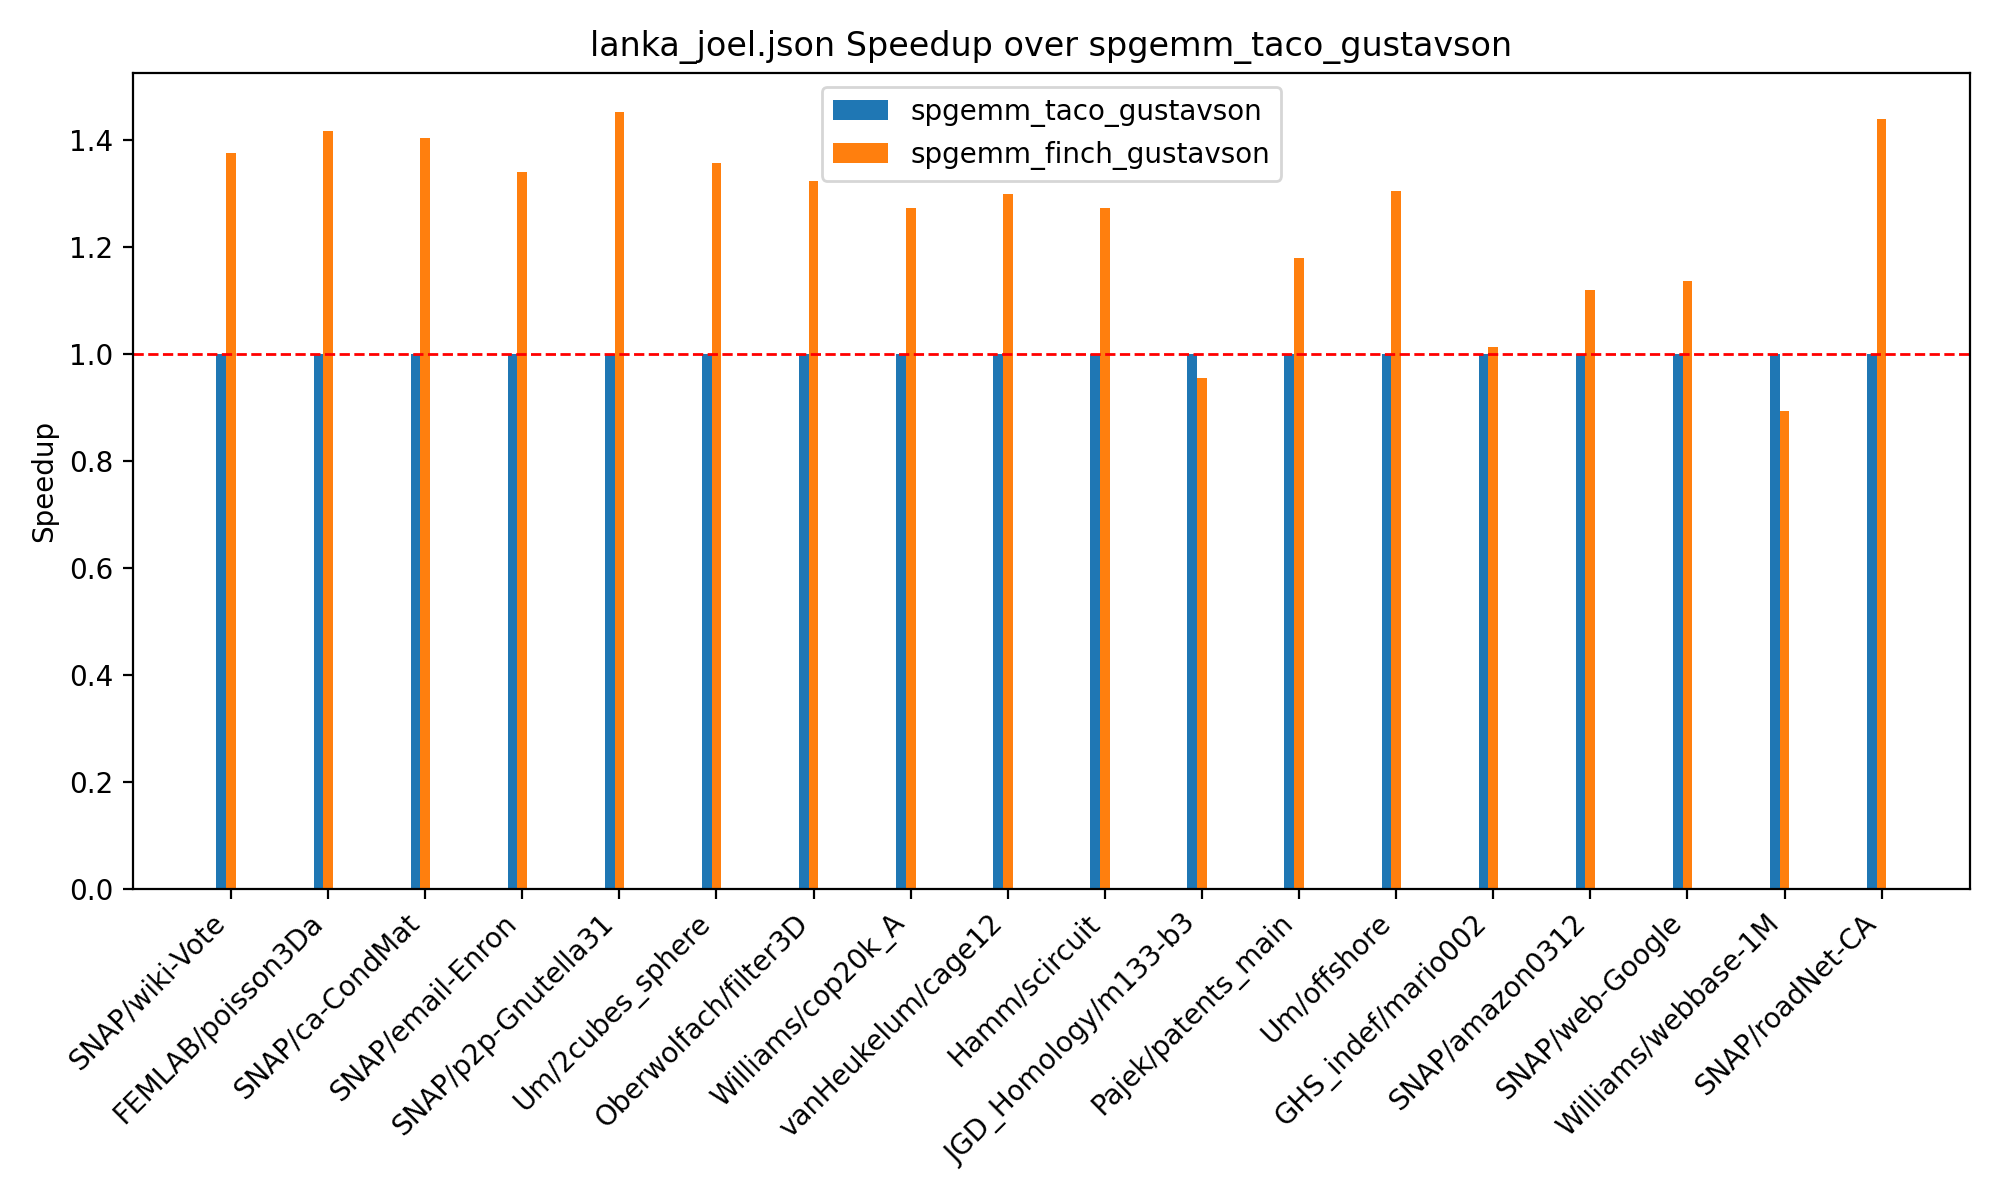
\includegraphics[width=\linewidth]{spgemm_joel_speedup.png}
    \caption{A comparison of gustavson's algorithm between Finch and Taco on some larger matrices}
\end{figure}

Examples that demonstrate performance engineering in a datastructure-driven model

\subsubsection{SpMV}
The sparse matrix-vector multiplication kernel (SpMV) is a common operation in sparse linear algebra with many applications including conjugate gradients, graph algorithms, numerical analysis, and neural networks [cite]. SpMV is a bandwidth bound kernel, and thus historically has been subject to many modifications to improve throughput and reduce the associated control flow [cite]. The wide range of applications unsurprisingly results in a wide range of types of datasets making it an effective kernel to demonstrate the utility of having flexible data formats. 

In this case study, we highlight a few different Finch formats as specified in Table \ref{spmv_tensor_formats}, and the performance effects of conforming a dataset’s structure with its storage format, which Finch's datastructure-driven model enables us to do. Finch also provides the control flow necessary to manipulate data reads and writes, enabling exploitation of multiple structural patterns concurrently (e.g. sparsity \textit{and} symmetry). 


We display speedup relative to TACO, SuiteSparseGraphBLAS, and Julia’s standard library, as depicted in Figures \ref{spmv_sorted} and \ref{spmv_grouped}.  We test using sparse matrices from a large selection of datasets spanning several previous papers: the datasets used by Vuduc et al. to test the OSKI interface [cite], Ahrens et al. to test a variable block row format partitioning strategy [cite], and Kjolstad et al. to test the TACO library [cite]. Additionally, we included the SNAP graph collection to test with boolean matrices. We also created several synthetic matrices containing bands or blocks of varying sizes as well as a permutation matrix to encapsulate a few additional use cases. The dense vector is randomly generated. We tested using the row-major and column-major Finch programs in Figure \ref{spmv_programs} as well as the symmetric program where applicable; the performance displayed for Finch on each dataset in Figure \ref{spmv_grouped} is the fastest among the formats and programs we tested. Column-major SpMV consistently performs better than row-major SpMV (an average of 1.36x better) in TACO so we use column-major SpMV in TACO as our baseline.

% TODO: make this be 3 columns
\begin{figure}
    \begin{minipage}[t]{0.315\textwidth}
        \vspace{0pt} % Add this to ensure top alignment within minipage
        \begin{minted}{julia}
            @finch begin
                y .= 0
                for j = _, i = _
                    y[i] += A[i, j] * x[j]
                end
                return y
            end
        \end{minted}
    \end{minipage}%
    \begin{minipage}[t]{0.315\textwidth}
        \vspace{0pt} % Add this to ensure top alignment within minipage
        \begin{minted}{julia}
            @finch begin
                y .= 0
                for j = _, i = _
                    y[j] += A[i, j] * x[i]
                end
                return y
            end
        \end{minted}
    \end{minipage}
    \begin{minipage}[t]{0.36\textwidth}
        \vspace{0pt} % Add this to ensure top alignment within minipage
        \begin{minted}{julia}
            @finch begin
                y .= 0
                for j = _
                    let x_j = x[j]
                        y_j .= 0
                        for i = _
                            let A_ij = A[i, j]
                                y[i] += x_j * A_ij
                                y_j[] += A_ij * x[i]
                            end
                        end
                        y[j] += y_j[] + diag[j] * x_j
                    end
                end
                return y
            end
        \end{minted}
    \end{minipage}
    \caption{Finch SpMV Programs}
    \label{spmv_programs}
\end{figure}



\begin{table}[htbp]
    \centering
    \caption{SpMV Tensor Formats}
    \label{spmv_tensor_formats}
    \begin{tabular}{|l|l|l|l|}
        \hline
        \textbf{Outer Level} & \textbf{Inner Level} & \textbf{Scalar Values} & \textbf{Style of Matrix}\\
        \hline
        \multirow{6}{*}{Dense} & \multirow{2}{*}{SparseList} & Element & sparse, real-valued matrices \\
        \cline{3-4} 
        & & Pattern & sparse, boolean-valued matrices \\
        \cline{2-4} 
        & SparseVBL & Element & real-valued matrices with blocked structure \\
        \cline{2-4}
        & SparseBand & Element & real-valued matrices with diagonal band \\
        \cline{2-4}
        & \multirow{2}{*}{SparsePoint} & Element & real-valued matrices with one value per row \\
        \cline{3-4} 
        & & Pattern & matrix with runs of true or false \\
        \hline 
    \end{tabular}
\end{table}



\subsubsection{Tensor Formats}
We found that the SpMV performance was superior for the level format that best paralleled the structure of the tensor. We consider the Dense(SparseList(Element)) format with the column-major SpMV program to be the Finch baseline as it is the closet analog to the sparse matrix format and SpMV program in other libraries.  

Namely, matrices with a clear blocked structure like exdata\_1, TSOPF\_RS\_b678\_c1, and heart3 performed notably well with the SparseVBL format with speedups of 2.16, 1.55, and 1.30 relative to TACO, while the baseline format had slowdowns of 0.71, 0.53, and 0.92 relative to TACO. Furthermore, the synthetic Toeplitz banded matrices we constructed performed the best with the SparseBand matrix, in particular with the toeplitz\_large\_band and the toeplitz\_medium\_band matrices having a speedup of 1.98 and 1.64 relative to TACO, while the baseline format had slowdowns of 0.84 and 0.51 relative to TACO.

There were also significant advantages of using the Pattern format instead of the Element format to represent scalar values in the matrices when these values were boolean, such as matrices in the SNAP collection which represent graph datasets are boolean. For example, the SparseList-Pattern for email-Eu-core resulted in a speedup of 2.51, while the SparseList-Element format resulted in a slowdown of 1.84 over TACO.

\begin{table}[htbp]
    \centering
    \caption{SpMV Sample Matrices}
    \label{spmv_sample_matrices}
    \begin{tabular}{|m{3cm}|c|c|c|}
        \hline
        \textbf{Spy} & \textbf{Group / Name} & \textbf{Dimensions} & \textbf{Best Finch Format}\\
        \hline
        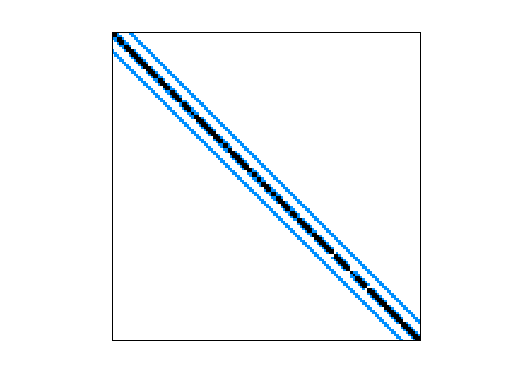
\includegraphics[width=3cm]{spmv_matrices/saylr4.png} & HB/saylr4 & 3,564 x 3,564 (22,316) & Symmetric SparseList \\
        \hline 
        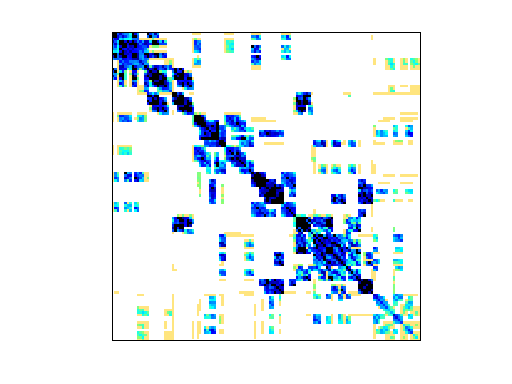
\includegraphics[width=3cm]{spmv_matrices/heart3.png} & Norris/heart3 & 2,339 x 2,339 (680,341) & SparseVBL \\
        \hline 
        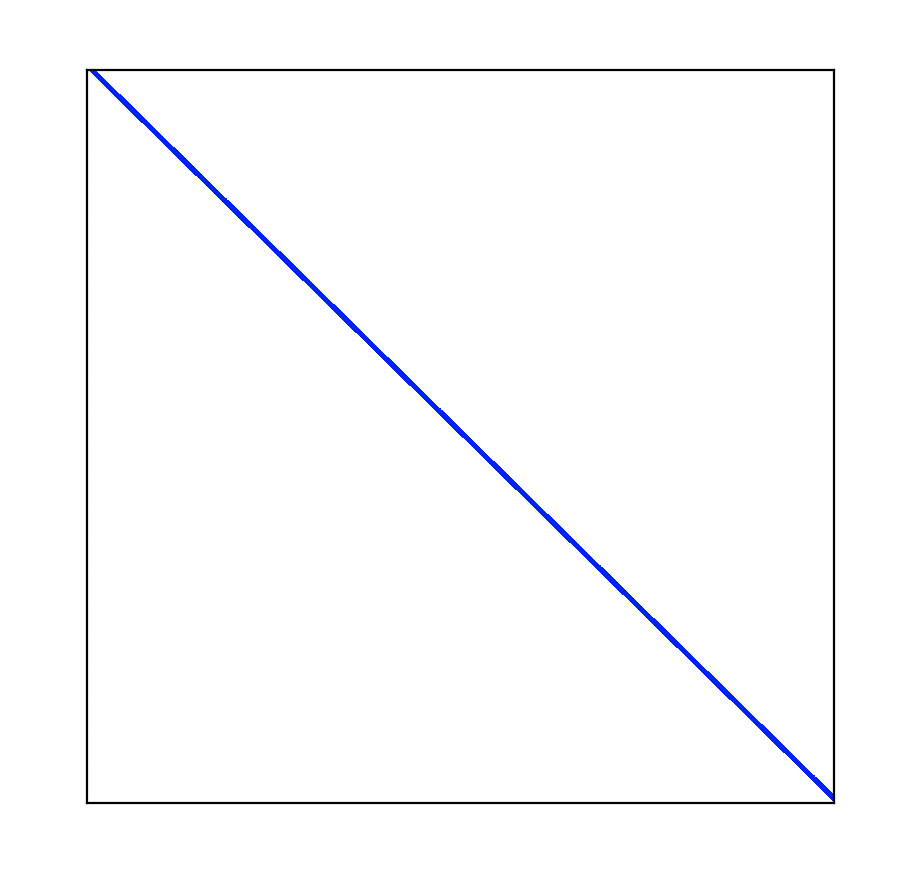
\includegraphics[width=3cm]{spmv_matrices/toeplitz_large_band.png} & toeplitz\_large\_band  & 10,000 x 10,000 (1,999,900) & SparseBand \\
        \hline
        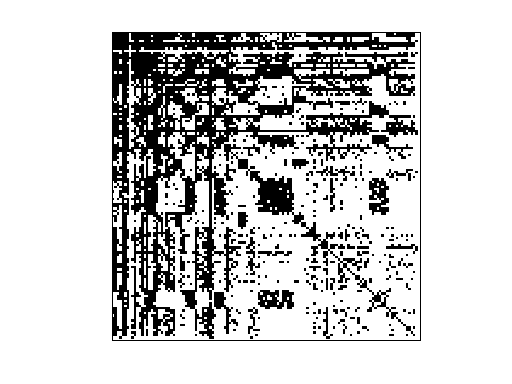
\includegraphics[width=3cm]{spmv_matrices/as-735.png} & SNAP/as-735 & 7,716 x 7,716 (26,467) & Symmetric SparseList-Pattern \\
        \hline
    \end{tabular}
\end{table}

\subsubsection{Symmetric SpMV}
Finch enables us to exploit symmetry in the sparse matrix of the SpMV kernel by providing the capabilities to reuse memory reads and insert control flow logic to restrict iterations to either the lower or upper triangle of the sparse matrix. We can apply this strategy with any level format. Every symmetric matrix in the SparseList and SparseList-Pattern formats has better performance when we use a Finch SpMV program that takes advantage of this symmetry. However, the regular row- or column-major Finch SpMV programs have better performance for symmetric matrices than the symmetric Finch SpMV program for the other more specialized formats, likely because we need in-order accesses to fully capitalize on the specialized storage. Symmetric SpMV with the SparseList level format in Finch results in an average of 1.27x speedup over TACO and symmetric SpMV with the SparseList-Pattern format in Finch results in an average speedup of 1.21x over TACO. Notably, there is a 1.91x speedup for the HB/saylr4 matrix over TACO. 

% Perhaps add the following section again in a future iteration of paper
% \subsubsection{4D Blocked SpMV}
% Finch also provides us the capability of writing an SpMV kernel [point to figure] that computes the output in blocks. Specifically, we rewrite an n x n matrix as a n/b x n/b x b x b 4-dimensional tensor and the vector as an n x n/b matrix where b is the block-size. We represent the blocked matrix with a SparseList as its second level (i.e. of format Dense(SparseList(Dense(Dense(Element(0.0)))))) so that only the non-zero blocks are stored. Then, we perform SpMV on each b x b block individually. Note that although SparseVBL already stores consecutive nonzeros in blocks, the benefit of a 4D-blocked kernel is that it additionally computes the output block by block. This method enables us to take advantage of spatial and temporal locality via register reuse [cite].

% We evaluated the 4D-blocked kernel on the Kronecker product of a neural network matrix (erdos-renyi, with sparsity p = ?) with a blocked matrix of size 10x10 and a dense and randomly generated vector. We found a 1.04x speedup to TACO, indicating comparable performance, and a 1.35x speedup to computing a non-blocked SpMV with the SparseVBL format, the fastest performing 2D Finch format for this matrix. 

% Structured matrices with induced dense blocks of equivalent size commonly arise in machine learning applications. In feature extraction, the Kronecker product of image data and a smaller matrix is computed to extract relevant features [cite]. Graph adjacency matrices or Laplacian matrices may also exhibit dense blocks when certain subsets of nodes or edges are densely interconnected. For instance, the adjacency matrix of the Erdös-Renyi random graph has a real symmetric bxb random block at each non-vanishing entry [cite]. 


%Here's a figure with spmv_performance_sorted_(faster_than_taco).png and spmv_performance_sorted_(slower_than_taco).png

\begin{figure}
    \begin{minipage}[t]{0.5\textwidth}
        \vspace{0pt} % Add this to ensure top alignment within minipage
        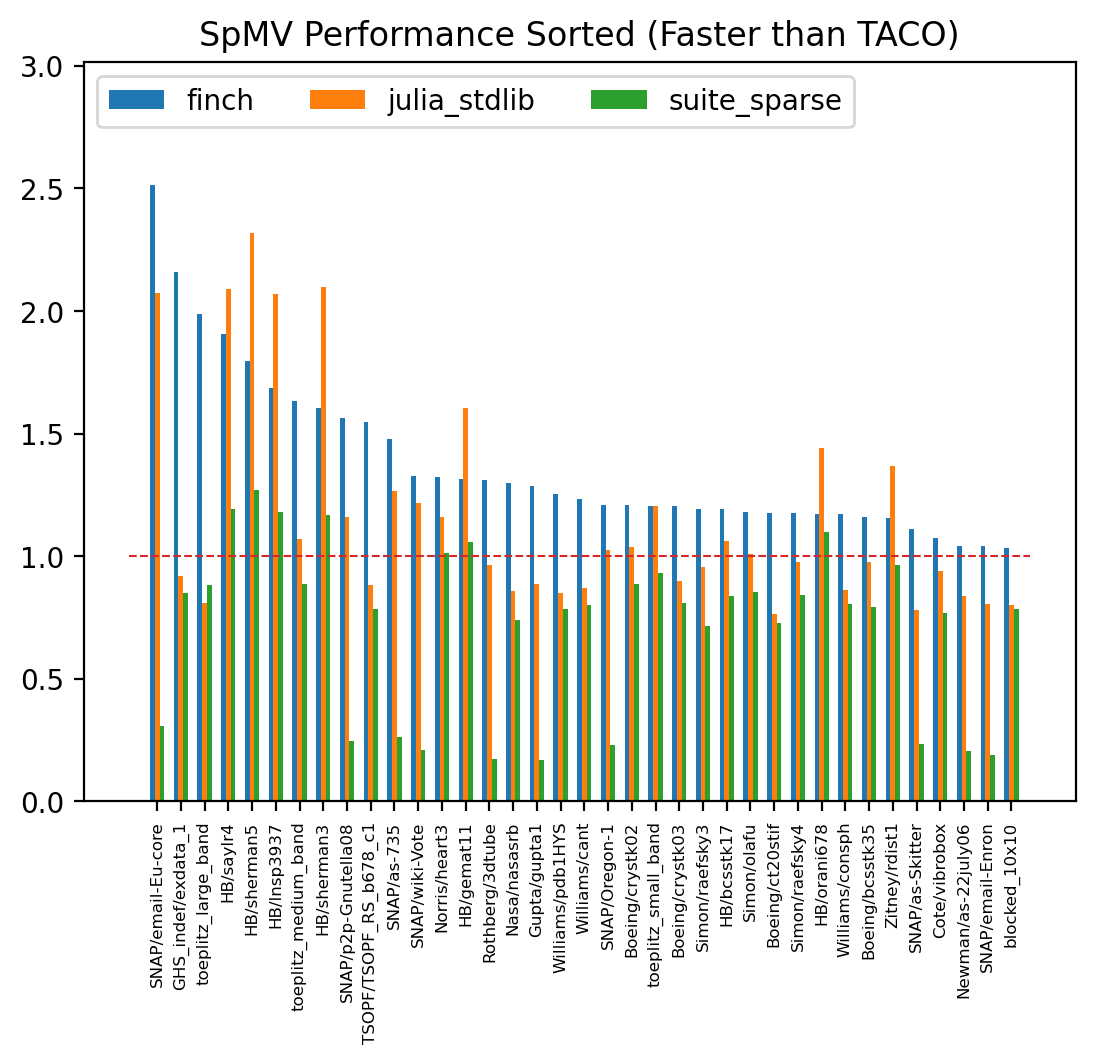
\includegraphics[width=\linewidth]{spmv_performance_sorted_(faster_than_taco).png}
    \end{minipage}%
    \begin{minipage}[t]{0.5\textwidth}
        \vspace{0pt} % Add this to ensure top alignment within minipage
        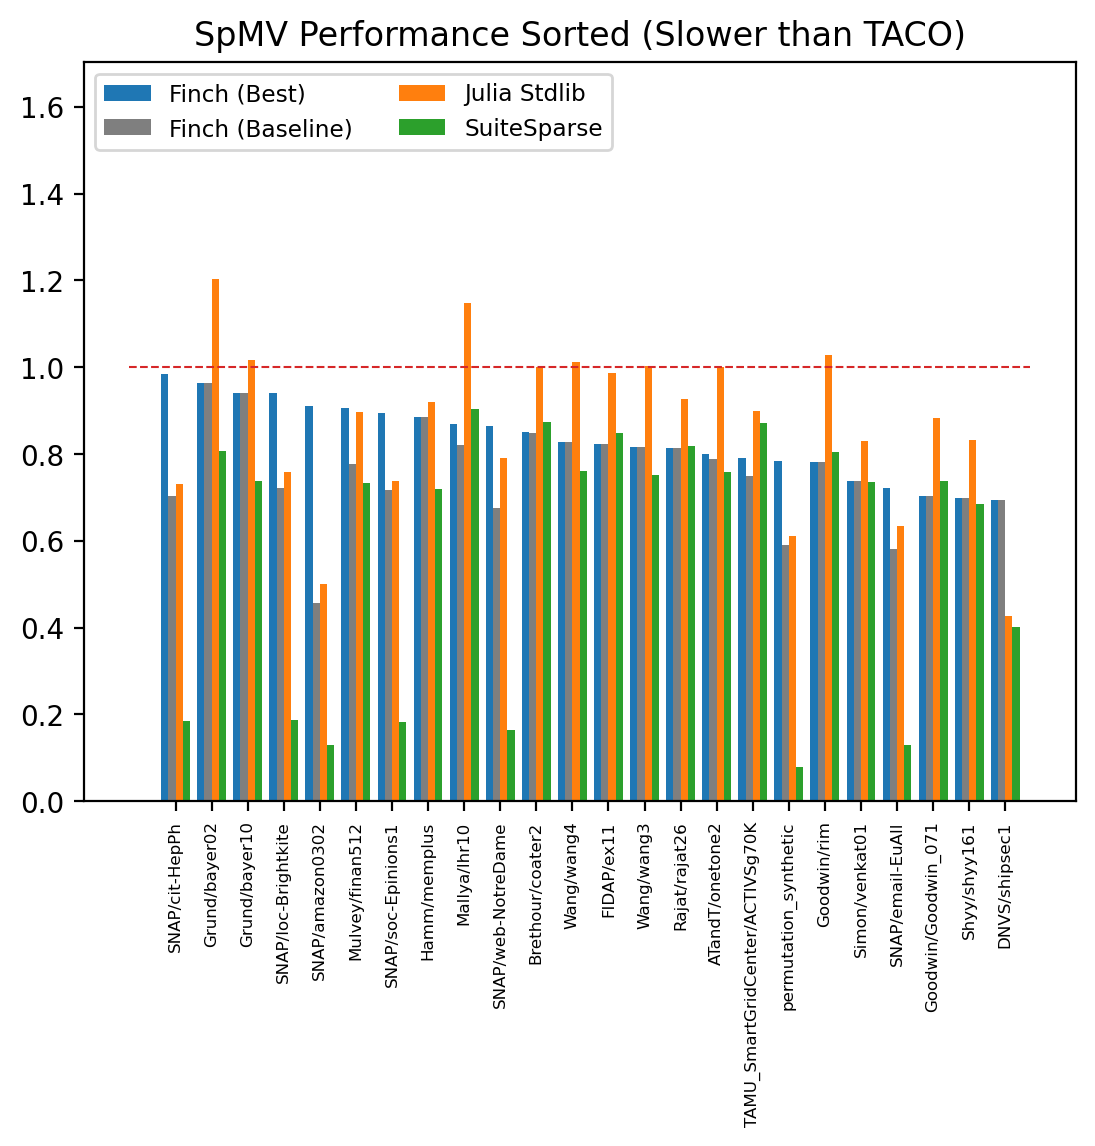
\includegraphics[width=\linewidth]{spmv_performance_sorted_(slower_than_taco).png}
    \end{minipage}
    \caption{Performance of SpMV across various tools.}
    \label{spmv_sorted}
\end{figure}

\begin{figure}
    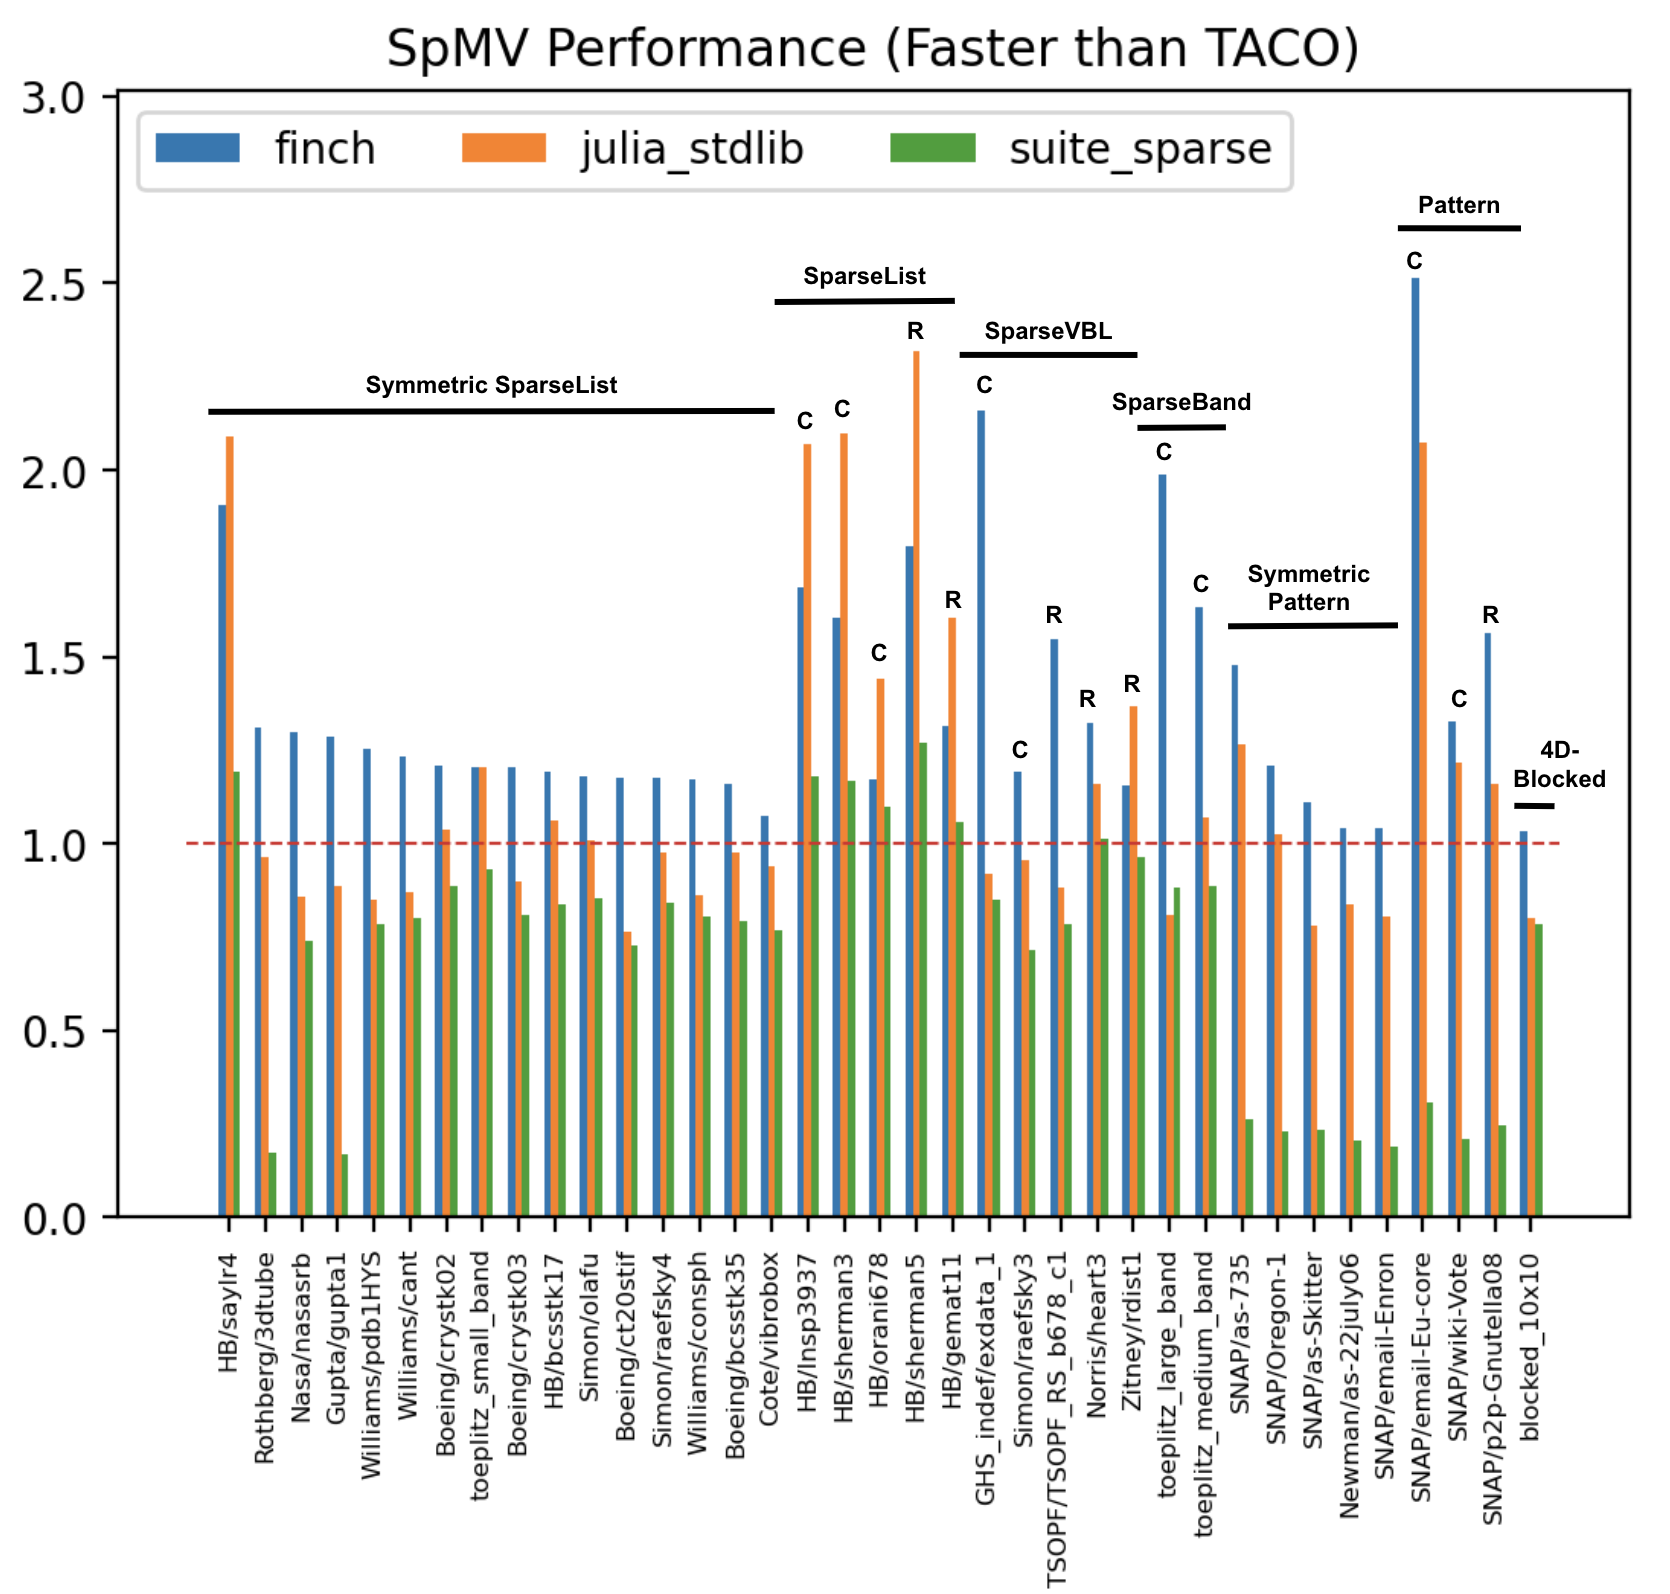
\includegraphics[width=\linewidth]{spmv_performance_grouped.png}
    \caption{Performance of SpMV by Finch format.}
    \label{spmv_grouped}
    \footnotesize The performance displayed for Finch on each dataset is the fastest among the formats we tested. "R" indicates row-major implementation and "C" indicates column-major implementation in Finch. The baseline Finch format is unsymmetric Dense(SparseList(Element)).
\end{figure}

\subsection{Programming over flexible data}

\subsubsection{Image Morphology}

\help{In this section, explain what erosion is, link a few cool images that show erosion, and then explain what the finch kernel looks like. in particular, be sure to point out that we're doing unrolled convolution, and how that maps to the generated code (merging shifted sparse iterators).}

\help{Explain the role of formats in this kernel, how sparseRLE(PAttern) is really the right thing to use here}

\help{Explain that finch can support a bitwise version, and that finch can mask the bitwise kernel too to get performance with a small change to the code}

\help{Point out that masks with SparseRLE can sometimes perform better because they lift the masking out of the inner loop. Talk about hist and also the fact that Finch supports scatter, here and in spgemm.}

\begin{figure}
	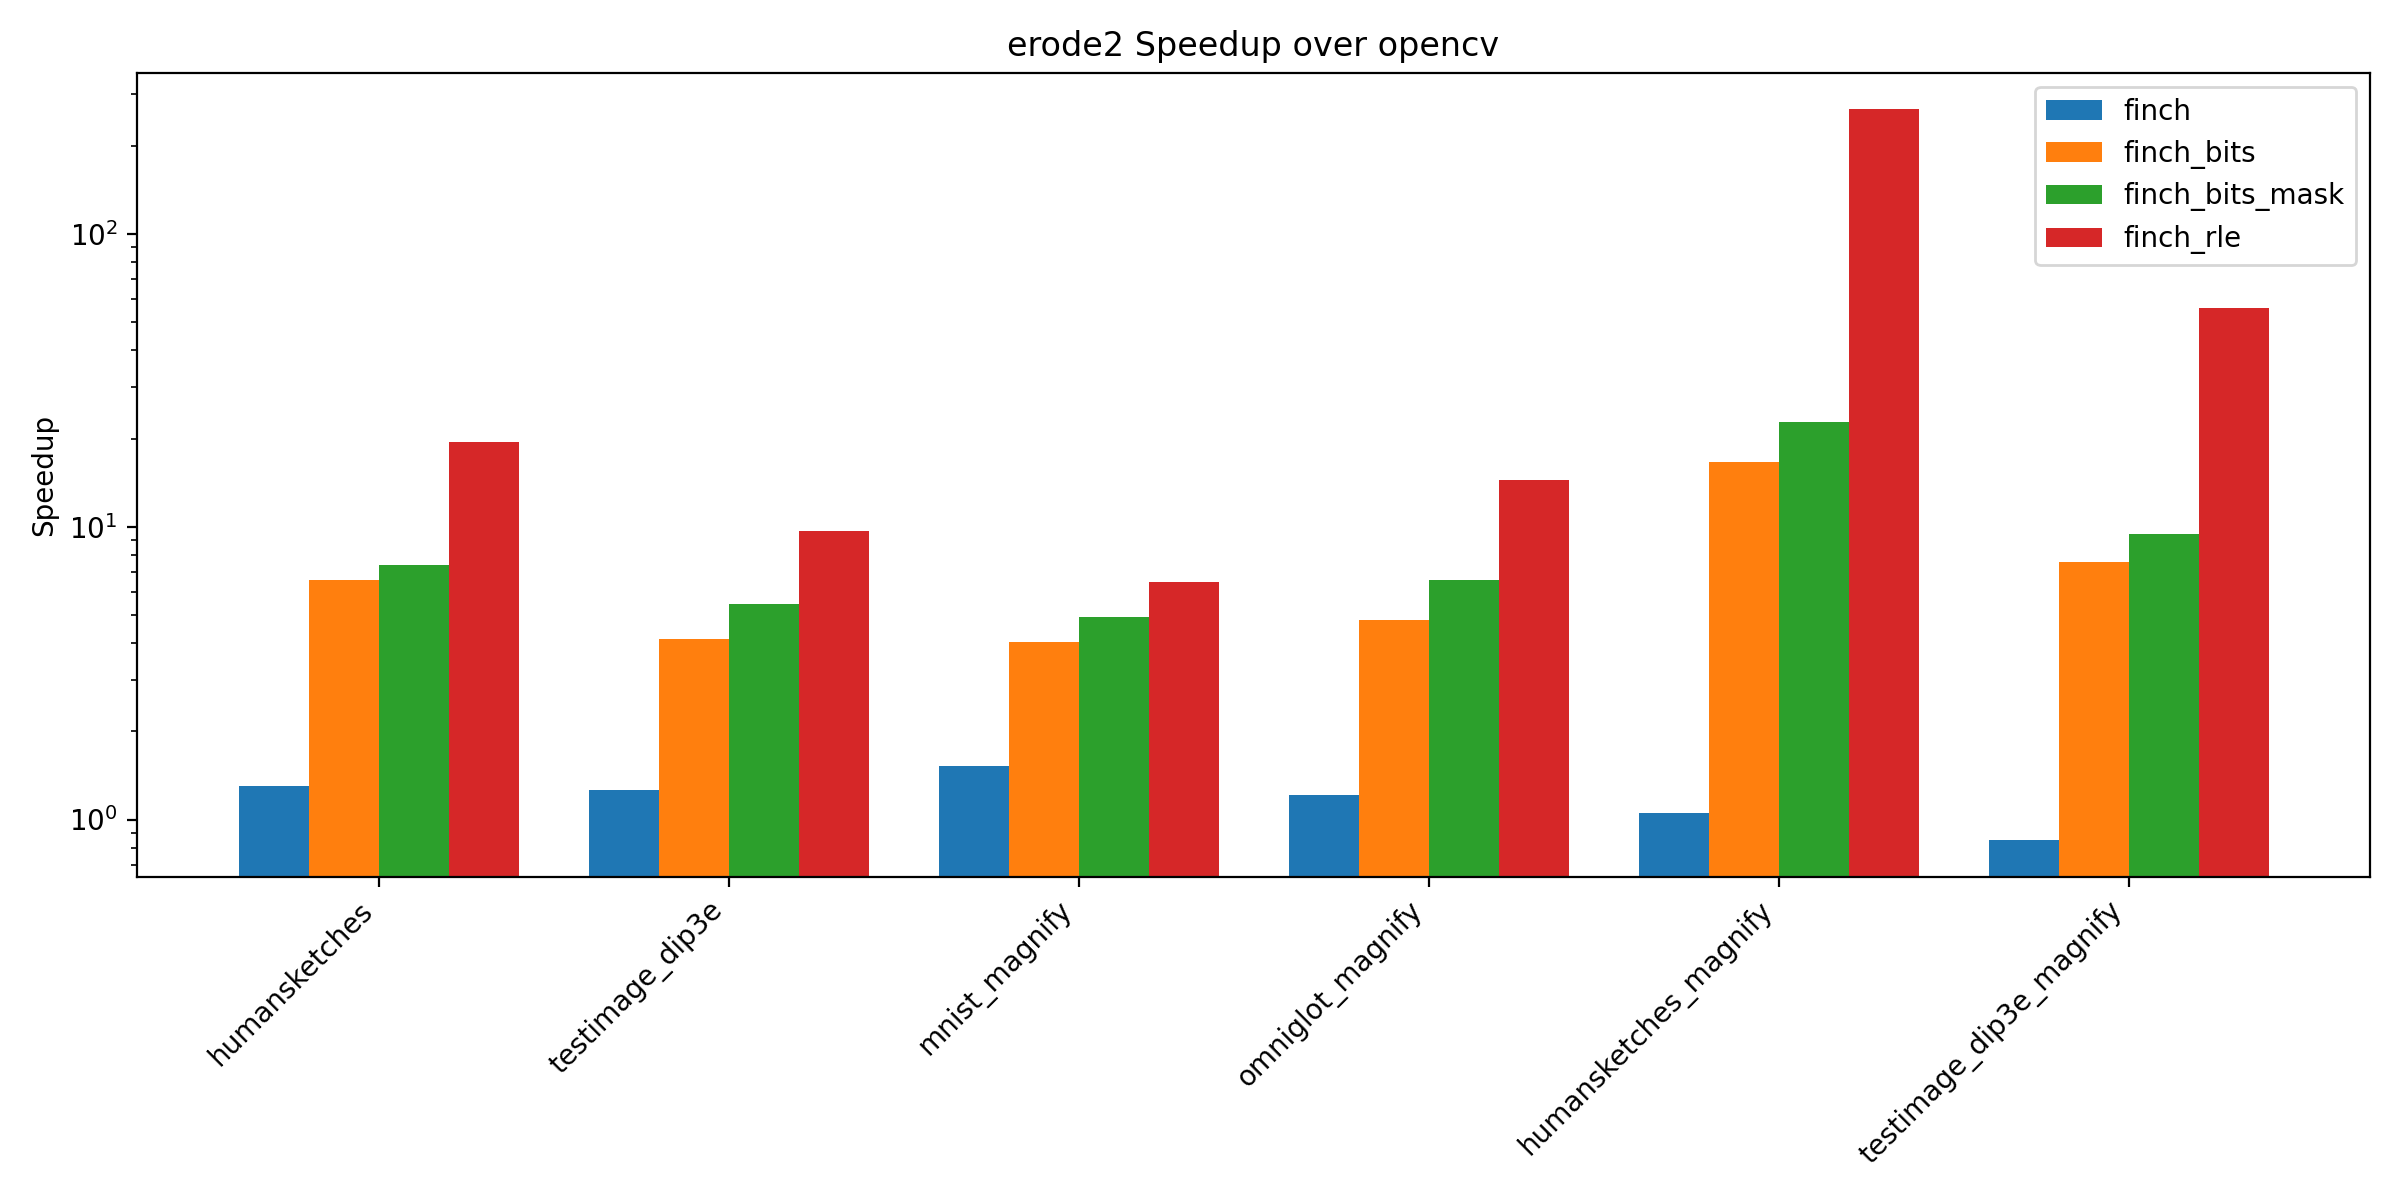
\includegraphics[width=\linewidth]{erode2_speedup_over_opencv.png}
    \caption{Performance of Finch on erosion task (2 iterations).}
\end{figure}

\begin{figure}
	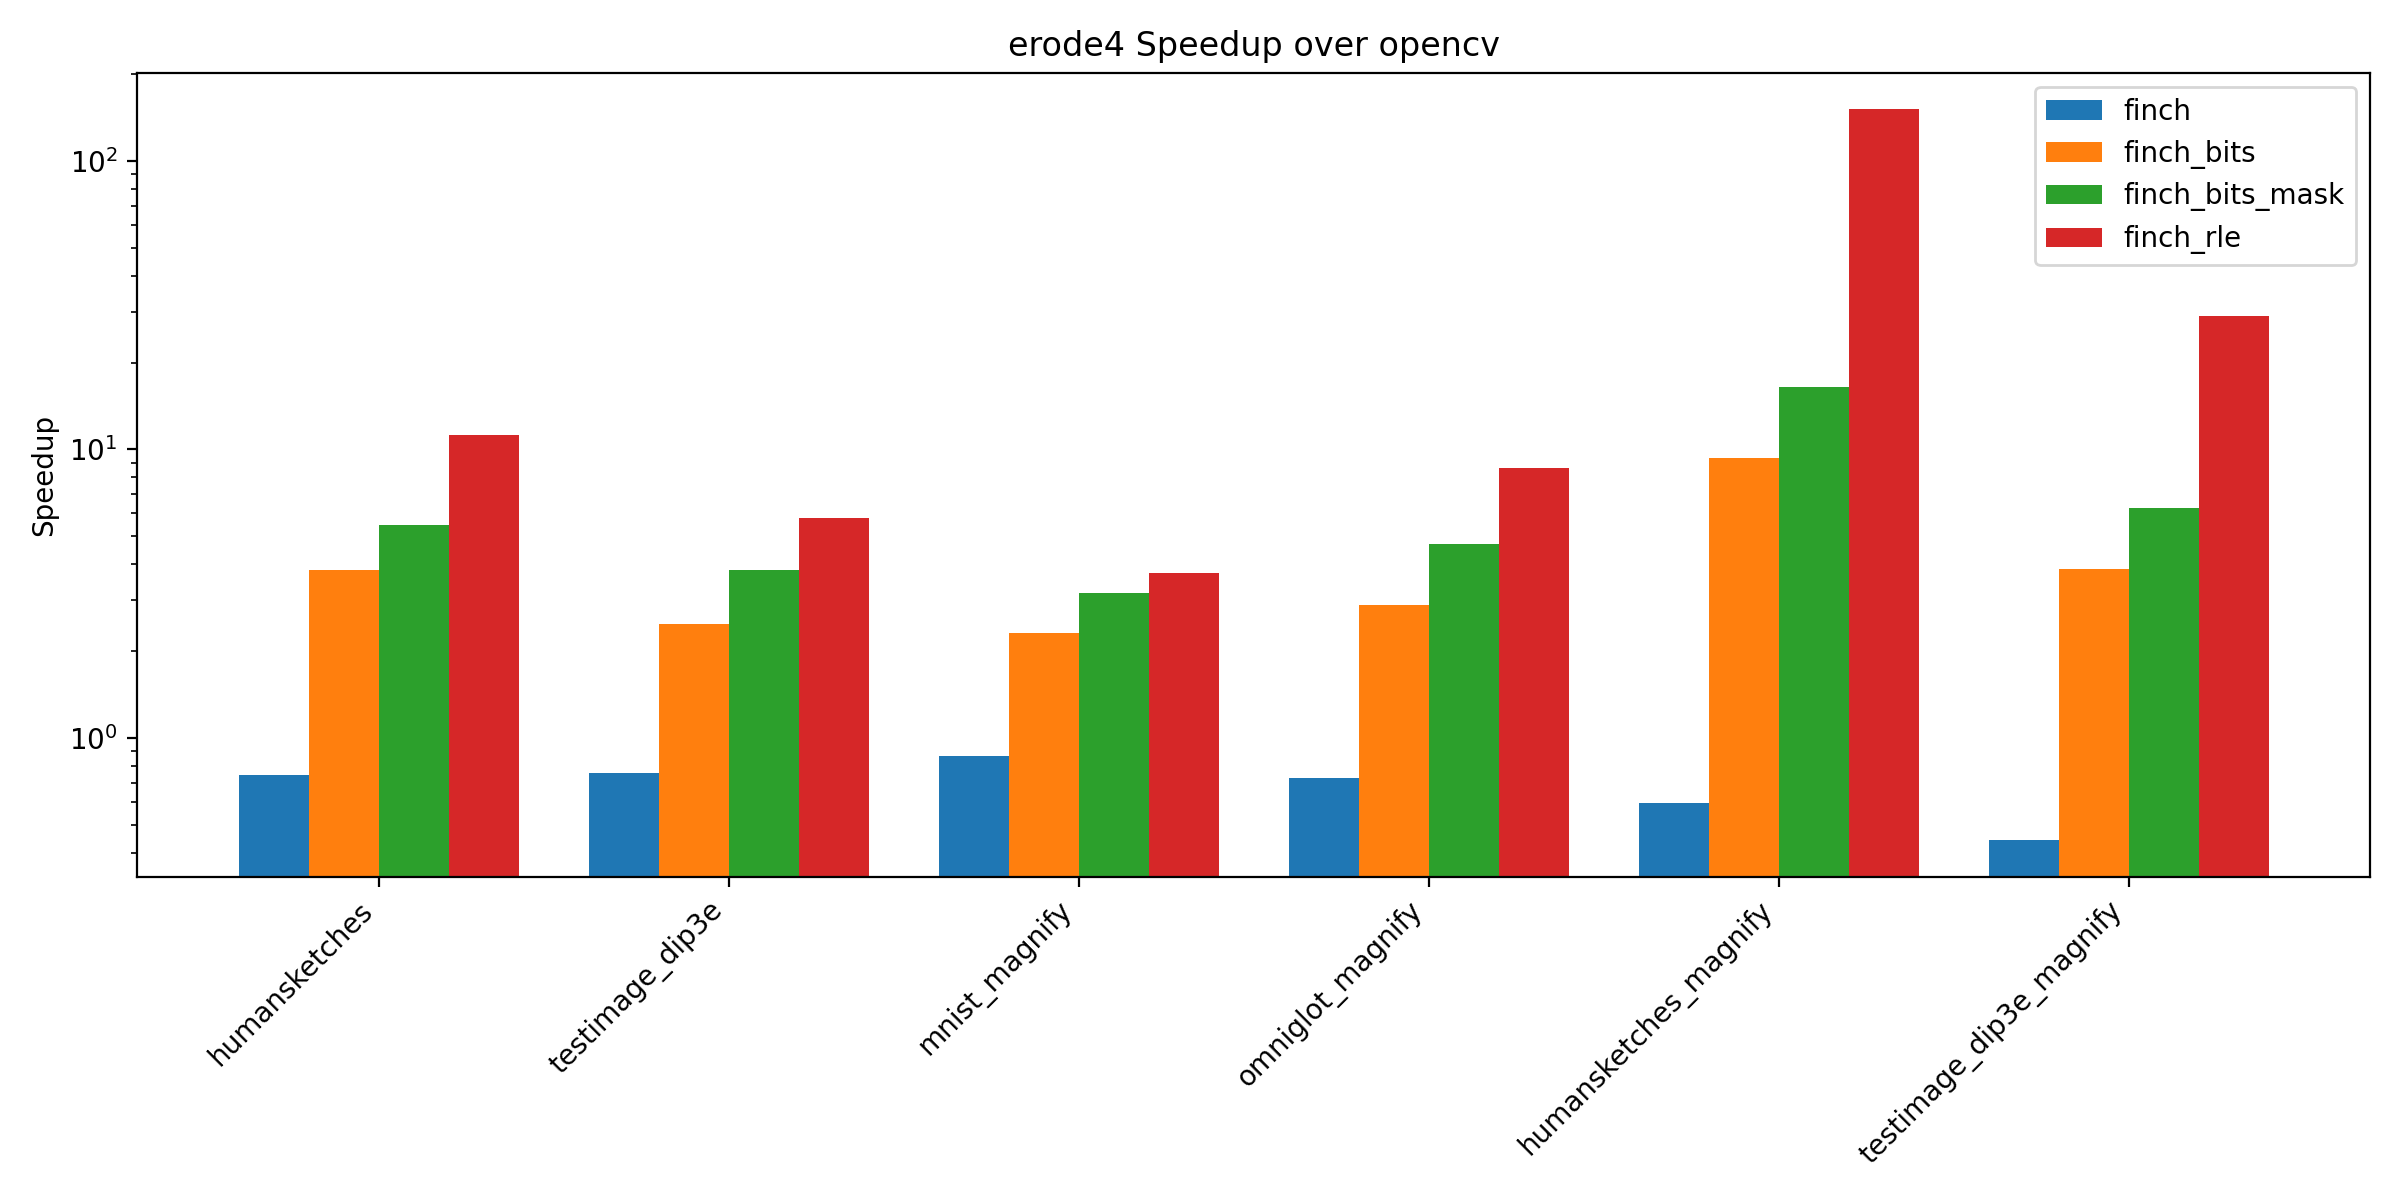
\includegraphics[width=\linewidth]{erode4_speedup_over_opencv.png}
    \caption{Performance of Finch on erosion task (4 iterations).}
\end{figure}

\begin{figure}
	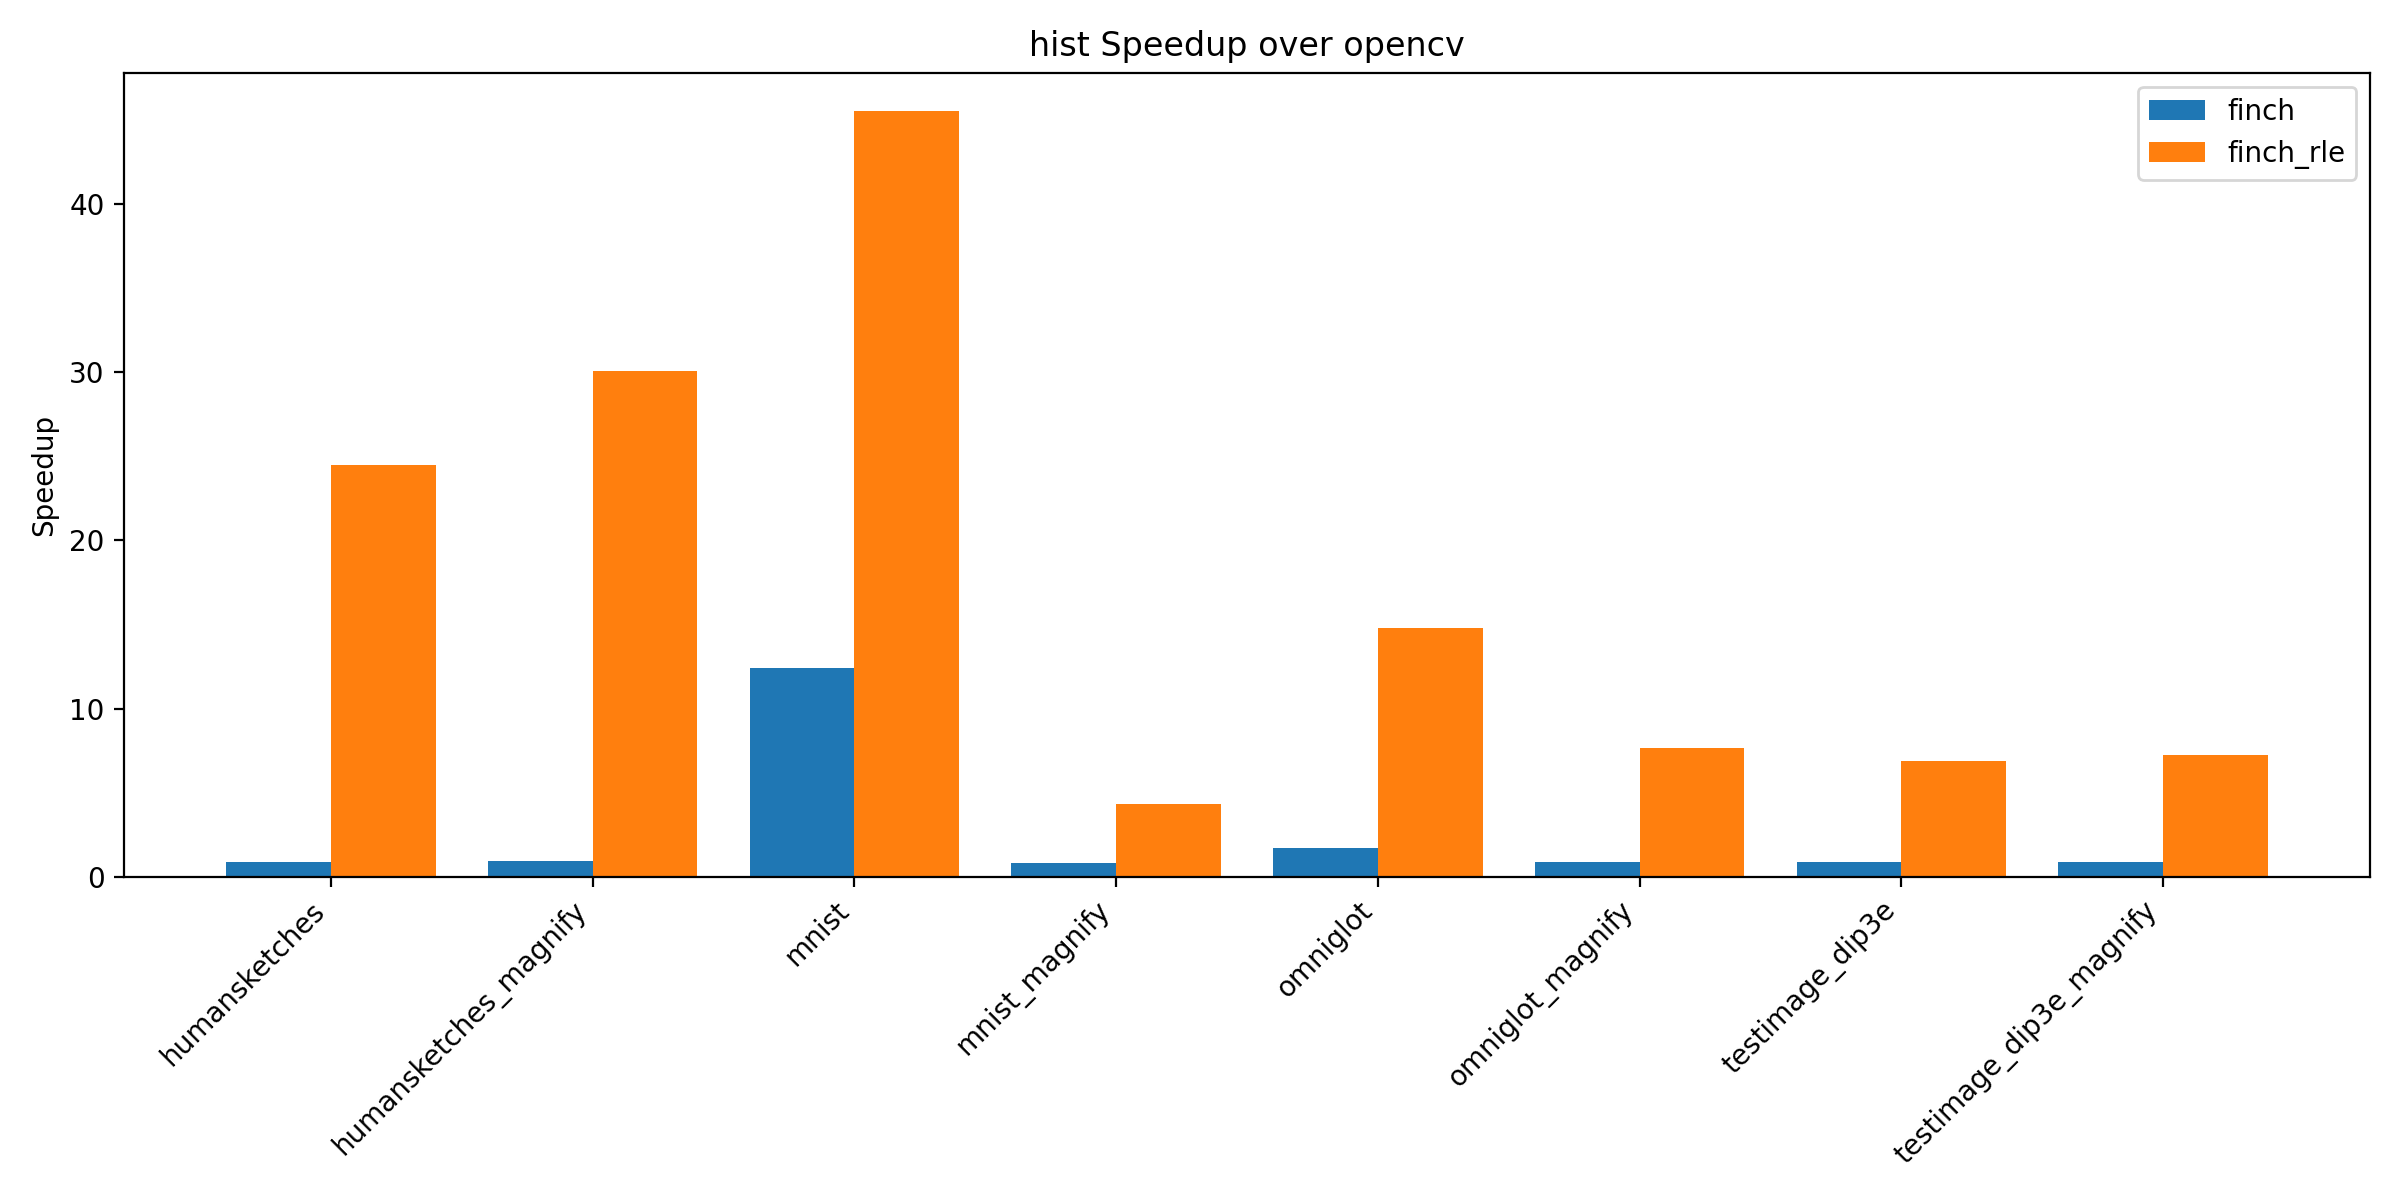
\includegraphics[width=\linewidth]{hist_speedup_over_opencv.png}
    \caption{Performance of Finch on masked histogram task.}
\end{figure}

\subsubsection{Graph Analytics}
\help{In this case, the two main highlights are that Finch can do arbitrary operators (i.e. choose), and that Finch can do early break, and also the different loop orders and multiple outputs. We may need to explain a little bit about what push pull is. For bellman, the main point is that we need multiple outputs, sparse inputs, masks, and sparse outputs with differing formats at differing points.}

\begin{figure}
	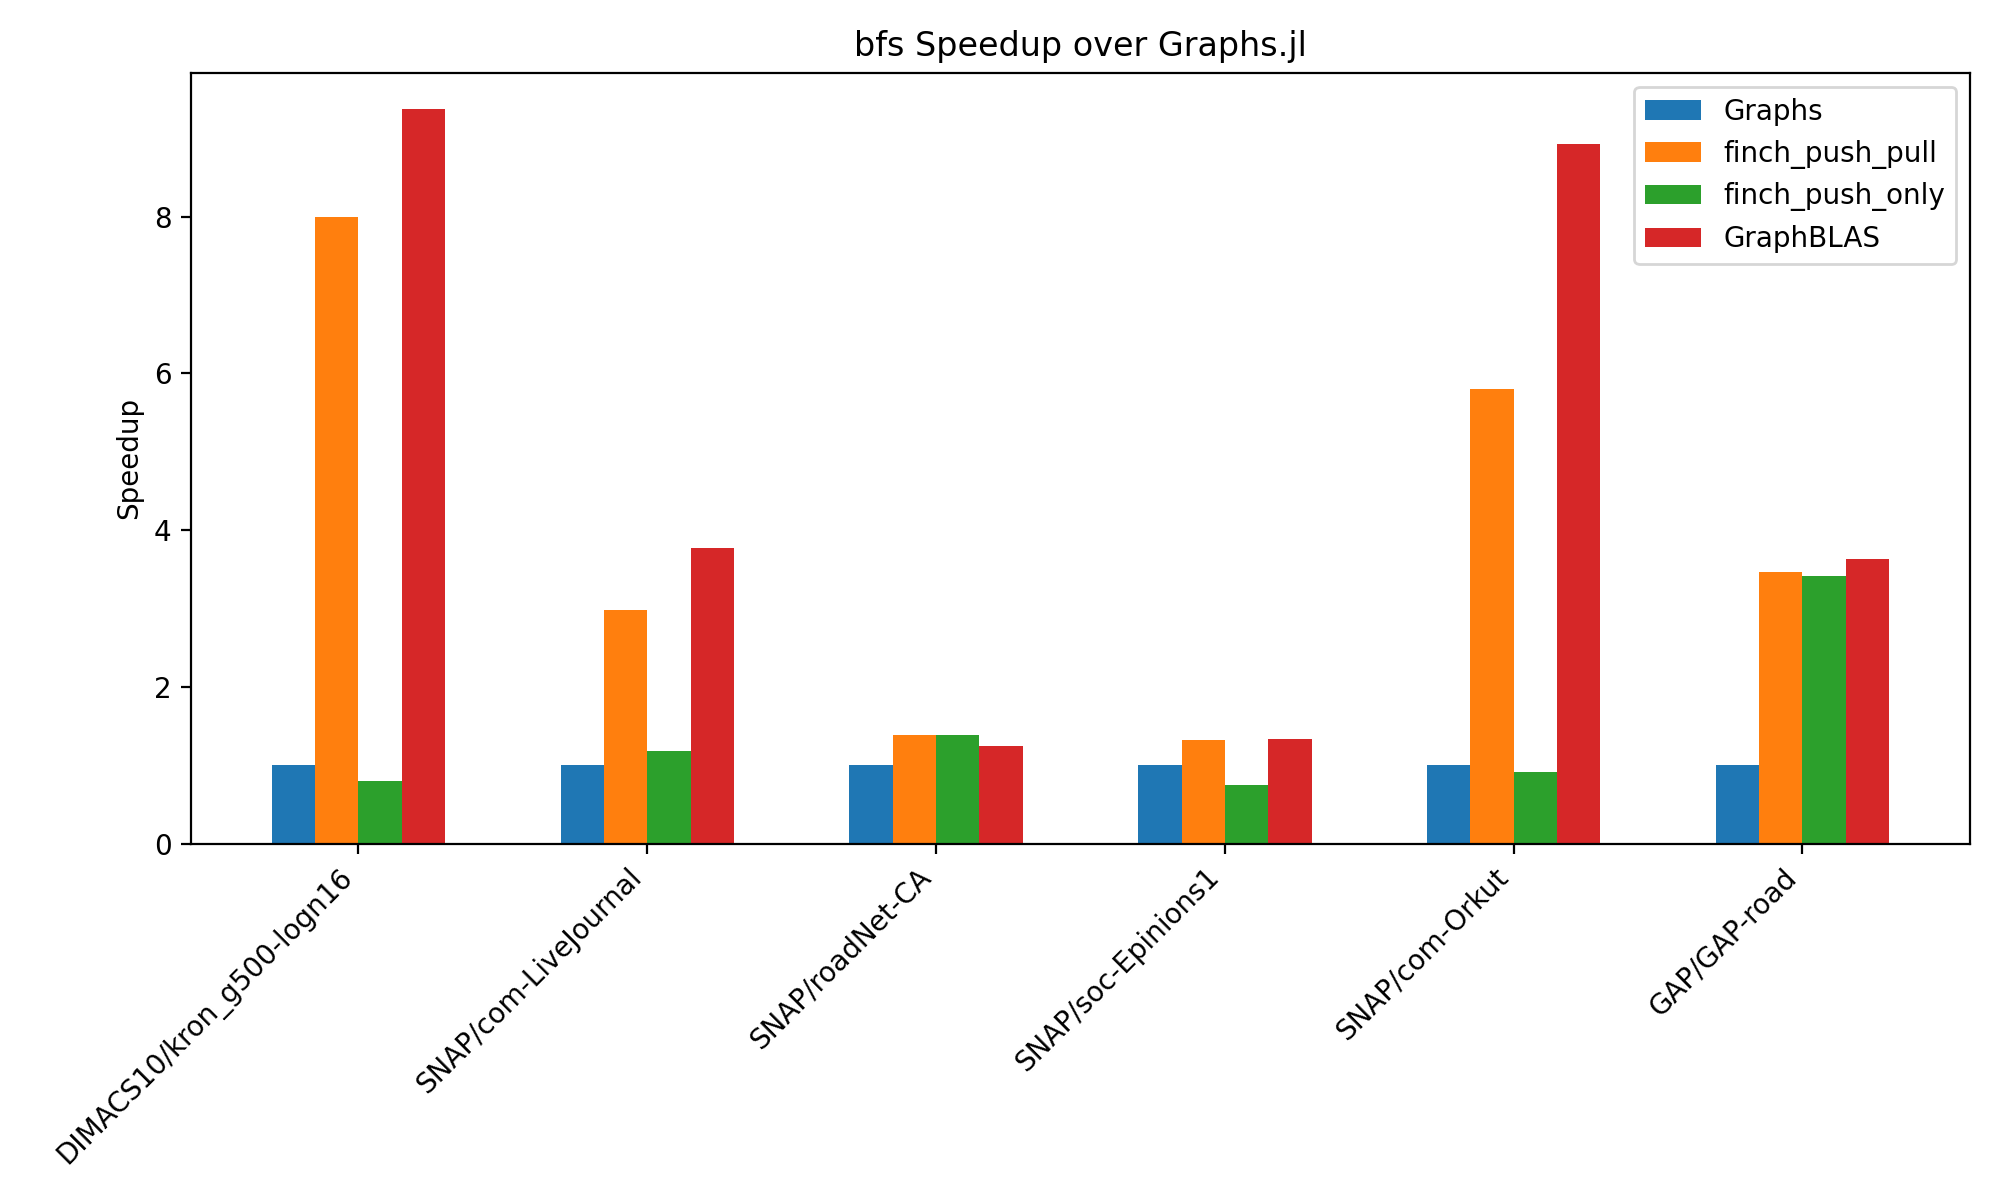
\includegraphics[width=\linewidth]{bfs_speedup_over_graphs.jl.png}
	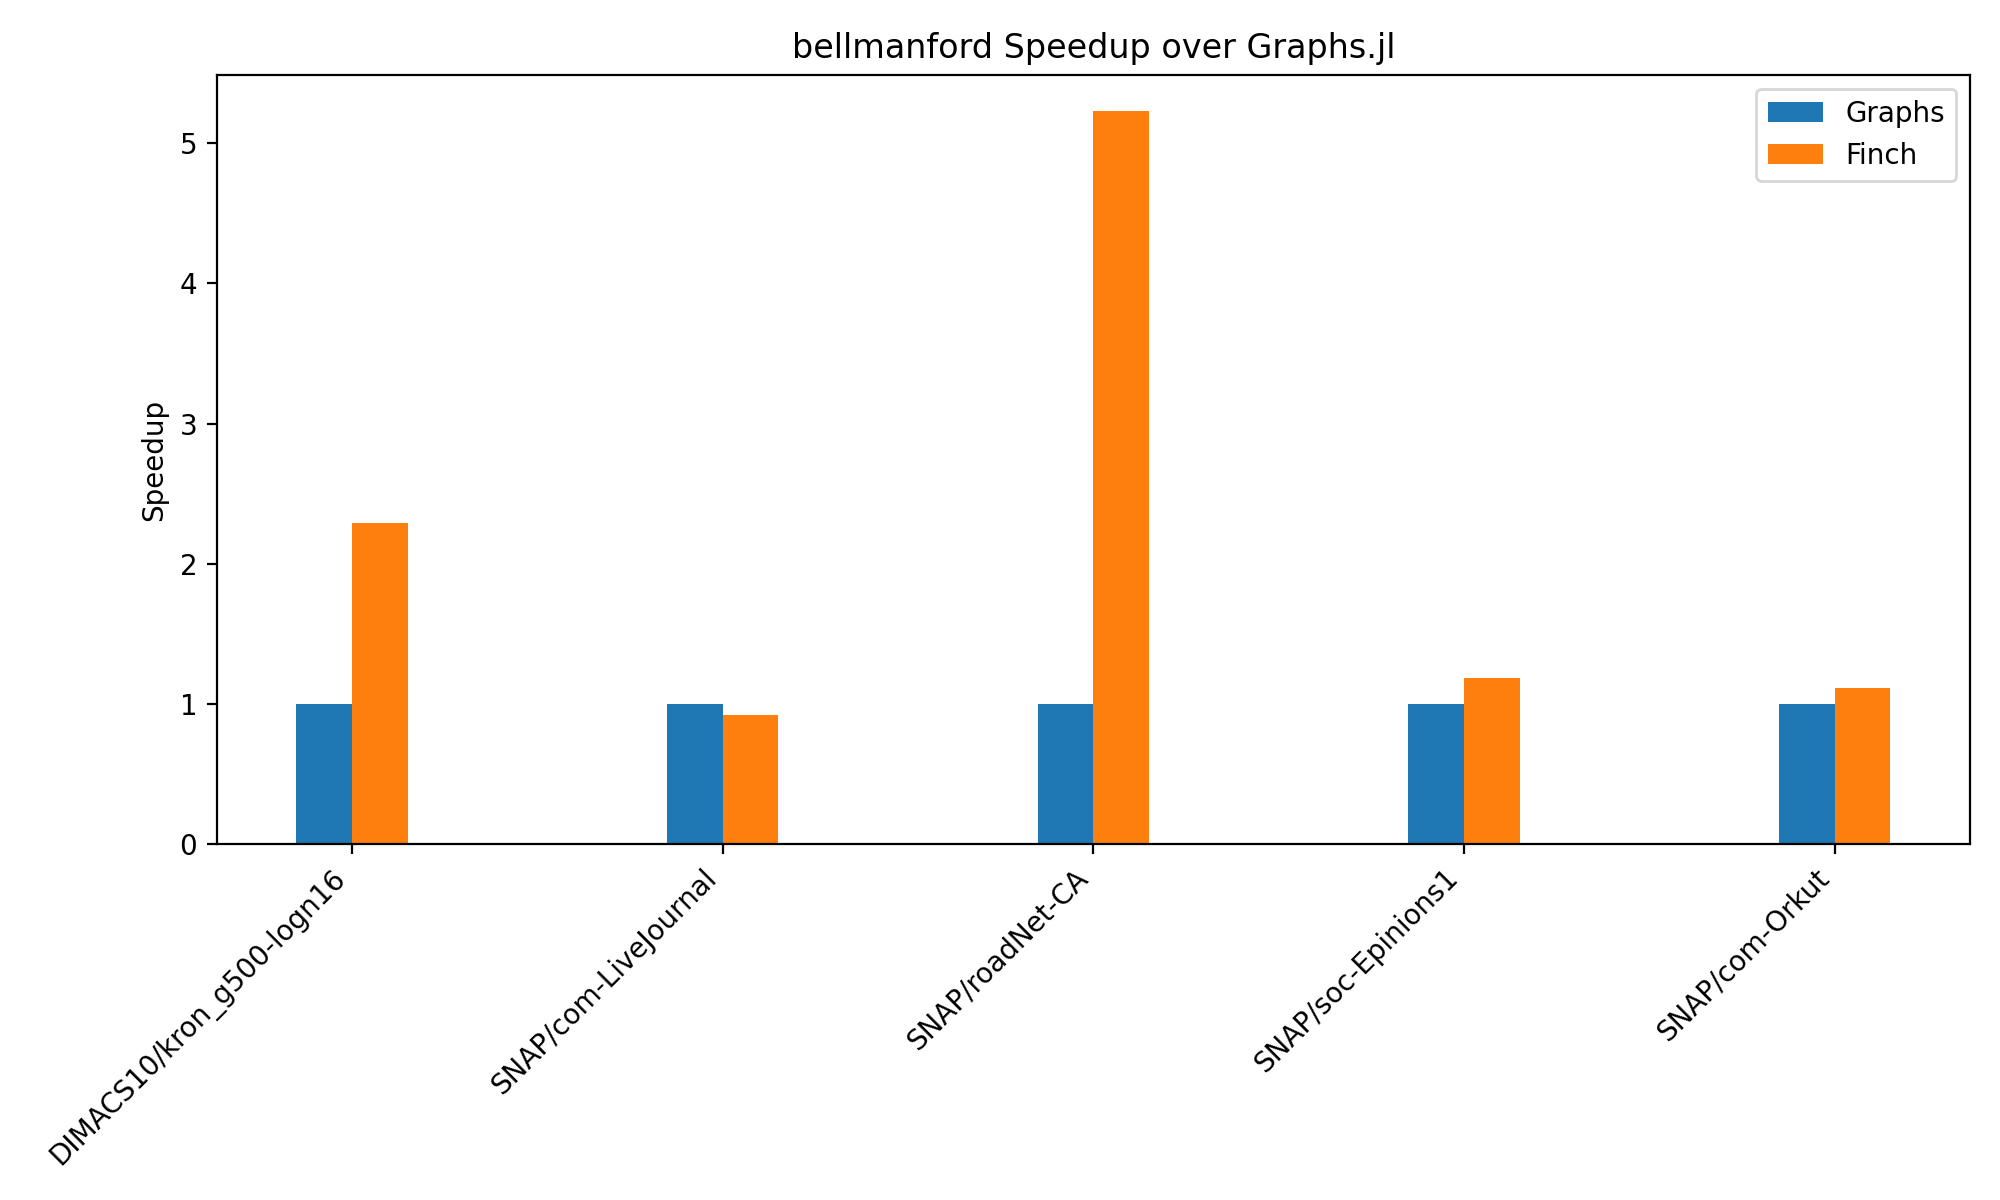
\includegraphics[width=\linewidth]{bellmanford_speedup_over_graphs.jl.png}
    \caption{Performance of graph apps across various tools.}
\end{figure}

Push-Pull BFS in Finch:
\begin{minted}{julia}
V = Tensor(Dense(Element(false)))
P = Tensor(Dense(Element(0)))
F = Tensor(SparseByteMap(Pattern()))
_F = Tensor(SparseByteMap(Pattern()))
A = Tensor(Dense(SparseList(Pattern())))
AT = Tensor(Dense(SparseList(Pattern())))

function finch_bfs_push_kernel(_F, F, A, V, P)
    @finch begin
        _F .= false
        for j=_, k=_
            if F[j] && A[k, j] && !(V[k])
                _F[k] |= true
                P[k] <<choose(0)>>= j #Only set the parent for this vertex
            end
        end
        return _F
    end
end


function finch_bfs_pull_kernel(_F, F, AT, V, P)
    p = ShortCircuitScalar{0}()
    @finch begin
        _F .= false
        for k=_
            if !V[k]
                p .= 0
                for j=_
                    if F[follow(j)] && AT[j, k]
                        p[] <<choose(0)>>= j #Only set the parent for this vertex
                    end
                end
                if p[] != 0
                    _F[k] |= true
                    P[k] = p[]
                end
            end
        end
        return _F
    end
end
\end{minted}

\subsection{Implementing Numpy's Array API in Finch}
In the past decade, the adoption of the Python Array API \cite{harris_array_2020} has allowed for a proliferation array programming systems, but existing implementations of this API for structured data suffer from either incompleteness or inefficiency. They generally either limit the dimensionality to vectors and matrices or only support tabular representations in order to reduce the complexity of interactions between different formats. Further, existing work doesn't support the fusion of arbitrary operators which can have a drastic impact on performance as we show in Fig. (\kyle{PUT FIG HERE}). We believe that a flexible, online compiler like Finch which can manage the complexity of arbitrary operations between inputs with a wide variety of formats is the secret ingredient needed to make the array API performant for structured data.

There is a gap between the expressiveness of the purely declarative Array API and the Finch language which defines both the output and the algorithm. The naive approach to solving this would be to explicitly define a mapping from each function in the API to a Finch program which eagerly produces the output. This approach results in a simple translation procedure but misses crucial opportunities for optimization across a chain of function calls and needlessly materializes large intermediate results. To avoid this, we have implemented a lazy evaluation approach that collects API calls and then computes output when requested by the user. This is implemented through 1) Finch Logic, a minimal, high-level language for expressing array operations and 2) the Finch Interpreter, which lowers Finch Logic programs to one or more Finch programs while making heuristic decisions about output format, loop ordering, and protocols.

\subsubsection{Finch Logic}
The Finch Logic language takes inspiration relational algebra 

\begin{align*}
    \finchplan(queries...) &  \quad\quad\quad \finchquery(name, expr) & \finchreorder(expr, idxs...)\\
    \finchrelabel(expr, idxs...)& \quad\quad\quad \finchmapjoin(op, exprs...)  & \finchaggregate(op, expr)\\
    \quad\quad\quad & \quad\quad\quad \finchtable(tns, idxs...)\quad\quad\quad  & \quad\quad\quad \\
\end{align*}



\subsubsection{Finch Interpreter}

\subsubsection{Lowering}

\subsubsection{Heuristic Optimization}

Find an example where fusing the python interface gives a big speedup over non-fused kernels.

%matmul, mttkrp, repeated ttm, triangle counting, multiple pointwise,
%in-place.
%dot((v^t .* u), w)) vs. 
%(v^t .* dot(u, w))
